\section{Nonlinear Optimization}

In this section we discuss the generic nonlinear optimization problem that forms the basis for the rest of the material presented in this class. We write the minimization problem as 
\begin{equation*}
\begin{aligned}
& \underset{\bm{x} \in \mathcal{X}}{\min}
& & f(\bm{x})
\end{aligned}
\end{equation*}
where $f$ is the cost function, usually assumed twice continuously differentiable, $x \in \R^n$ is the optimization variable, and $\mathcal{X} \subset \R^n$ is the constraint set. The special case in which the cost function is linear and the constraint set is specified by linear equations and/or inequalities is \textit{linear optimization}, which we will not discuss. 

\subsection{Unconstrained Nonlinear Optimization}

We will first address the unconstrained case, in which $\mathcal{X} = \R^n$. A vector $\bm{x}$ is said to be an unconstrained \textit{local minimum} if there exists $\epsilon > 0$ such that $f(\bm{x}^*) \leq f(\bm{x})$ for all $\bm{x} \in \{\bm{x} \mid \|\bm{x} - \bm{x}^*\| \leq \epsilon\}$, and $\bm{x}$ is said to be an unconstrained \textit{global minimum} if $f(\bm{x}^*) \leq f(\bm{x})$ for all $x \in \R^n$. 

\subsubsection{Necessary Conditions for Optimality}

For a differentiable cost function, we can compare the cost of a point to its neighbors by considering a small variation $\Delta \bm{x}$ from $\bm{x}^*$. By using Taylor expansions, this yields a first order cost variation
\begin{equation}
    f(\bm{x}^* + \Delta \bm{x}) - f(\bm{x}^*) \approx \nabla f(\bm{x}^*)^T \Delta \bm{x}
\end{equation}
and a second order cost variation 
\begin{equation}
    f(\bm{x}^* + \Delta \bm{x}) - f(\bm{x}^*) \approx \nabla f(\bm{x}^*)^T \Delta \bm{x} + \frac{1}{2} \Delta \bm{x}^T \nabla^2 f(\bm{x}^*) \Delta \bm{x}.
\end{equation}
Setting $\Delta \bm{x}$ to be equal to positive and negative multiples of the unit coordinate vector, we have 
\begin{equation}
    \frac{\partial f(\bm{x}^*)}{\partial x_i} \geq 0
\end{equation}
where $x_i$ denotes the $i$'th coordinate of $\bm{x}$, and 
\begin{equation}
    \frac{\partial f(\bm{x}^*)}{\partial x_i} \leq 0
\end{equation}
for all $i$, which is only satisfied by $f(\bm{x}^*) = 0$.  This is referred to as the \textit{first order necessary condition for optimality}. Looking at the second order variation, and noting that $f(\bm{x}^*) = 0$, we expect
\begin{align}
f(\bm{x}^* + \Delta \bm{x}) - f(\bm{x}^*) \geq 0
\end{align}
and thus
\begin{align}
\Delta \bm{x}^T \nabla^2 f(\bm{x}^*) \Delta \bm{x} \geq 0
\end{align}
which implies $\nabla^2 f(\bm{x}^*)$ is positive semidefinite. This is referred to as the \textit{second order necessary condition for optimality}. Stating these conditons formally, 

\begin{theorem}[Necessary Conditions for Optimality (NOC)]
Let $\bm{x}^*$ be an unconstrained local minimum of $f:\R^n \to \R$ and $f \in C^1$ in an open set $S$ containing $\bm{x}^*$. Then
\begin{equation}
    \nabla f(\bm{x}^*) = 0.
\end{equation}
If $f \in C^2$ within $S$, $\nabla^2 f(\bm{x}^*)$ is positive semidefinite. 
\end{theorem}

Proof is given in Section 1.1 of \cite{bertsekas2016nonlinear}.

\subsubsection{Sufficient Conditions for Optimality}


\begin{figure}[t]
    \centering
    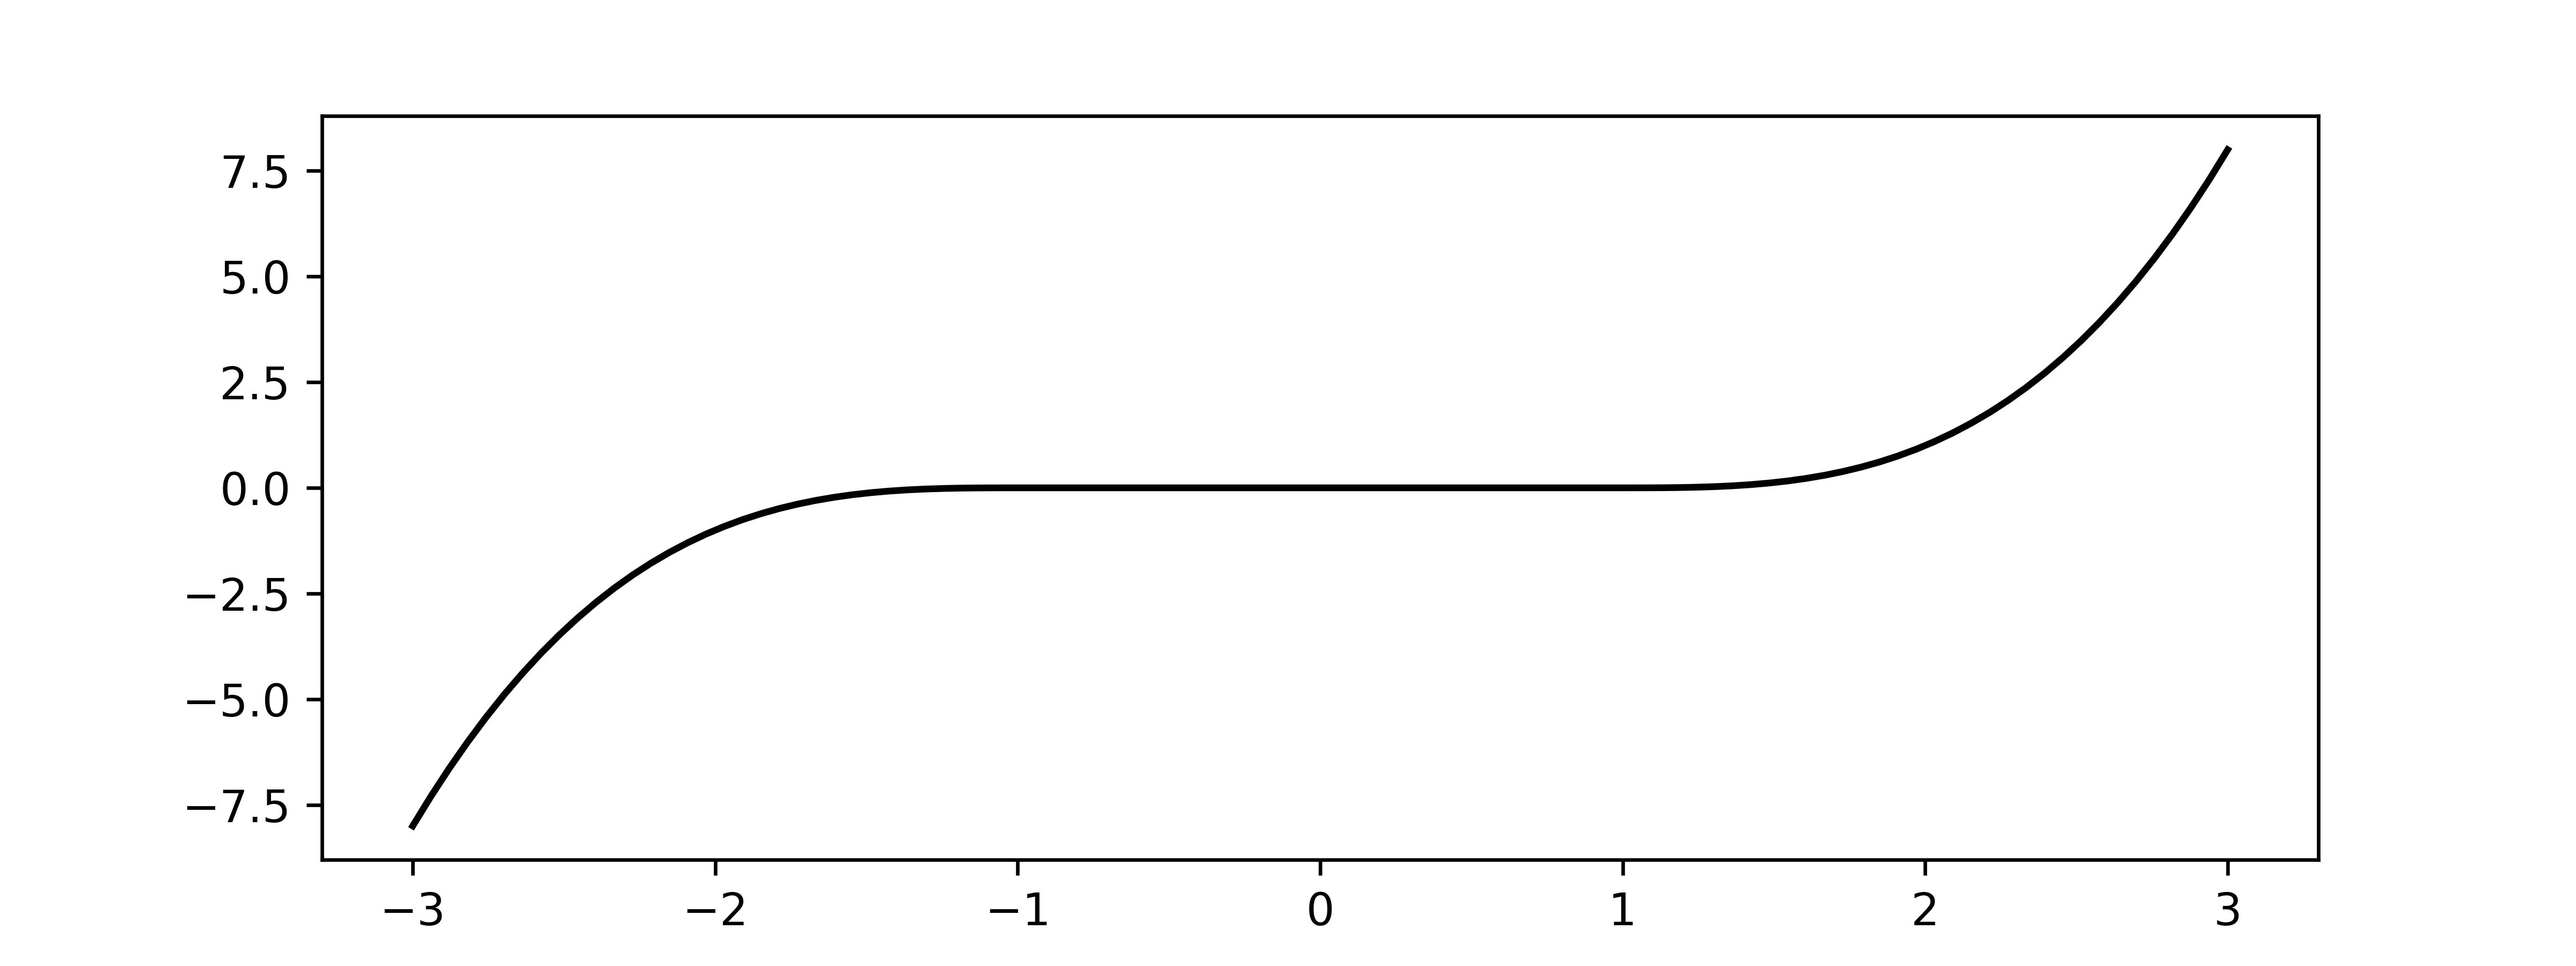
\includegraphics[width=0.85\linewidth]{figs/foc.png}
    \caption{An example of a function for which the necessary conditions of optimality are satisfied but the sufficient conditions are not.}
    \label{fig:foc}
\end{figure}


If we strengthen the second order condition to $\nabla^2 f(\bm{x}^*)$ being positive definite, we have the sufficient conditions for $\bm{x}^*$ being a local minimum. Why is the second order necessary conditions not sufficient? An example function is given in figure \ref{fig:foc}. Formally, 

\begin{theorem}[Sufficient Conditions for Optimality (SOC)]
Let $f:\R^n \to \R$ be $C^2$ in an open set $S$. Suppose a vector $\bm{x}^*$ satisfies the conditions $\nabla f(\bm{x}^*) = 0$ and $\nabla^2 f(\bm{x}^*)$ is positive definite. Then $\bm{x}^*$ is a strict unconstrained local minimum of $f$. 
\end{theorem}

Proof is again given in Section 1.1 of \cite{bertsekas2016nonlinear}.
There are several reasons why the optimality conditions are important. In a general nonlinear optimization setting, they can be used to filter candidates for global minima. They can be used for sensitivity analysis, in which the sensitivity of $\bm{x}^*$ to model parameters can be quantified \cite{bertsekas2016nonlinear}. This is common in e.g. microeconomics. Finally, these conditions often provide the basis for the design and analysis of optimization algorithms.

\subsubsection{Special case: Convex Optimization}

A special case within nonlinear optimization is the set of \textit{convex optimization} problems. A set $S \subset \R^n$ is called \textit{convex} if 
\begin{equation}
    \alpha \bm{x} + (1 - \alpha) \bm{y} \in S, \quad \forall \bm{x},\bm{y} \in S, \forall \alpha \in [0,1].
\end{equation}
For $S$ convex, a function $f:S\to\R$ is called convex if 
\begin{equation}
    f(\alpha \bm{x} + (1-\alpha) \bm{y}) \leq \alpha f(\bm{x}) + (1-\alpha) f(\bm{y}).
    \label{eq:conv_fun}
\end{equation}
This class of problems has several important characteristics. If $f$ is convex, then
\begin{itemize}
    \item A local minimum of $f$ over $S$ is also a global minimum over $S$. If in addition $f$ is strictly convex (the inequality in (\ref{eq:conv_fun}) is strict), there exists at most one global minimum of $f$.
    \item If $f \in C^1$ and convex, and the set $S$ is open, $\nabla f(\bm{x}^*) = 0$ is a necessary and sufficient condition for a vector $\bm{x}^* \in S$ to be a global minimum over $S$.
\end{itemize}
Convex optimization problems have several nice properties that make them (usually) computationally efficient to solve, and the first property above gives a certificate of having obtained global optimality that is difficult or impossible to obtain in the general nonlinear optimization setting. For a thorough treatment of convex optimization theory and algorithms, see \cite{boyd2004convex}. 

\subsubsection{Computational Methods}

In this subsection we will discuss the class of algorithms known as \textit{gradient methods} for finding local minima in nonlinear optimization problems. These approaches, rely (roughly) on following the gradient of the function ``downhill'', toward the minima. More concretely, these algorithms rely on taking steps of the form
\begin{equation}
    \bm{x}^{k+1} = \bm{x}^k + \alpha^{k} \bm{d}^k
\end{equation}
where if $\nabla f(\bm{x}) \neq 0$, $\bm{d}^k$ is chosen so that 
\begin{equation}
    \nabla f(\bm{x})^T \bm{d}^k < 0
\end{equation}
and $\alpha > 0$. Typically, the step size $\alpha^k$ is chosen such that 
\begin{equation}
    f(\bm{x}^k + \alpha^k \bm{d}^k) < f(\bm{x}^k),
\end{equation}
but generally, the step size and the direction of descent ($\bm{d}^k$) are tuning parameters. 

We will look at the general class of descent directions of the form 
\begin{equation}
    \bm{d}^k = -D^k \nabla f(\bm{x}^k)
\end{equation}
where $D^k > 0$ (note that this guarantees $\nabla f(\bm{x}^k)^T \bm{d}^k < 0$). 

\paragraph{Steepest descent, $D^k = I$.} The simplest choice of descent direction is directly following the gradient, and ignoring second order function information. In practice, this often leads to slow convergence and possible oscillation.

\paragraph{Newton's Method, $D^k = (\nabla^2 f(\bm{x}^k))^{-1}$.} The underlying idea of this approach is to at each iteration, minimize the quadratic approximation of $f$ around $\bm{x}^k$,
\begin{equation}
    f^k(\bm{x}) = f(\bm{x}^k) + \nabla f(\bm{x}^k)^T (\bm{x} - \bm{x}^k) + \frac{1}{2} (\bm{x} - \bm{x}^k)^T \nabla^2 f(\bm{x}^k) (\bm{x} - \bm{x}^k).
\end{equation}
Setting the derivative of this to zero, we obtain 
\begin{equation}
    \nabla f(\bm{x}^k) + \nabla^2 f(\bm{x}^k) (\bm{x} - \bm{x}^k) = 0
\end{equation}
and thus, by setting $\bm{x}^{k+1}$ to be the $\bm{x}$ that satisfies the above, we get the
\begin{equation}
    \bm{x}^{k+1} = \bm{x}^k - (\nabla^2 f(\bm{x}^k))^{-1} \nabla f(\bm{x}^k)
\end{equation}
or more generally, 
\begin{equation}
    \bm{x}^{k+1} = \bm{x}^k - \alpha (\nabla^2 f(\bm{x}^k))^{-1} \nabla f(\bm{x}^k).
\end{equation}
Note that this update is only valid for $\nabla^2 f(\bm{x}^k) > 0$. When this condition doesn't hold, $\bm{x}^{k+1}$ is not a minimizer of the second order approximation (as a result of the SOCs). 

\paragraph{Diagonally scaled steepest descent, $D^k = \textrm{diag}(d_1^k, \ldots, d_n^k)$.} Have $d_i^k >0 \forall i$. A popular choice is 
\begin{equation}
    d_i^k = \left( \frac{\partial^2 f(\bm{x}^k)}{\partial x_i^2} \right)^{-1}
\end{equation}
which is a diagonal approximation of the Hessian. 

\paragraph{Modified Newton's method, $D^k = (\nabla^2 f(\bm{x}^0))^{-1}$.} Requires $\nabla^2 f(\bm{x}^0) > 0$. For cases in which one expects $\nabla^2 f(\bm{x}^0) \approx \nabla^2 f(\bm{x}^k)$, this removes having to compute the Hessian at each step. 

In addition to choosing the descent direction, there also exist a variety of methods to choose the step size $\alpha$. A computationally intensive but efficient (in terms of the number of steps taken) is using a minimization rule of the form 
\begin{equation}
\alpha^k = \argmin_{\alpha\geq 0} f(\bm{x}^k + \alpha \bm{d}^k)  
\end{equation}
which is usually solved via line search. Alternative approaches include a limited minimization rule, in which you constrain $\alpha^k \in [0,s]$ during the line search, or simpler approach such as a constant step size (which may not guarantee convergence), or a diminishing scheduled step size. In this last case, schedules are typically chosen such that $\alpha^k \to 0$ as $k \to \infty$, while $\sum_{k=0}^\infty \alpha^k = +\infty$.

\subsection{Constrained Nonlinear Optimization}